\documentclass{article}
\usepackage[utf8]{inputenc}
\usepackage[T1]{fontenc} % behövs annars är underscore fula hm. kanske
\usepackage{caption}
\usepackage[swedish]{babel}
\usepackage{graphicx}
\usepackage{float}
\usepackage[colorlinks=true, allcolors=blue]{hyperref}
\usepackage{siunitx}
\usepackage{soul} % for the command \hl
\usepackage{listings}
\usepackage{xcolor}
\usepackage{circuitikz}

\definecolor{codegreen}{rgb}{0,0.6,0}
\definecolor{codegray}{rgb}{0.5,0.5,0.5}
\definecolor{codepurple}{rgb}{0.58,0,0.82}
\definecolor{backcolour}{rgb}{0.985,0.985,0.985}

\lstdefinestyle{mystyle}{
    backgroundcolor=\color{backcolour},   
    commentstyle=\color{codegreen},
    keywordstyle=\color{magenta},
    numberstyle=\tiny\color{codegray},
    stringstyle=\color{codepurple},
    basicstyle=\ttfamily\footnotesize,
    breakatwhitespace=false,         
    breaklines=true,                 
    captionpos=b,                    
    keepspaces=true,                 
    numbers=left,                    
    numbersep=5pt,                  
    showspaces=false,                
    showstringspaces=false,
    showtabs=false,                  
    tabsize=2
}

\lstset{style=mystyle}

% \newcommand{\kursnamn}{Sensorer, AI och inbyggda system 4 hp}
% \newcommand{\kurskod}{CC2018}
% \newcommand{\provkod}{2201}

\newcommand{\kursnamn}{Digitalisering inom tillverknings\-industrin, 20 YH-poäng}
\newcommand{\kurskod}{Produktionsteknik}
\newcommand{\provkod}{}

\begin{document}

  
\includegraphics[width=0.3\textwidth]{figures/HH_ENG_color_small.pdf}
  \hspace{3cm}
  
\includegraphics[width=0.4\textwidth]{figures/novalogga.jpg}

  \vspace{5mm}
	\begin{center}
	{\Huge{}Lab. 3 -- Maskininlärning}
	\end{center}
\noindent\rule{\textwidth}{2pt}
\\


{\Large
\begin{tabular}{p{2cm}p{1cm}p{8cm}}
&  &  \\
Kurs: & 	& 	\kursnamn \\
Kurskod: & & \kurskod \\
Provkod: &  & \provkod \\
L\"arare: &  & Pererik Andreasson \& Fredrik Lundborg\\
Uppdaterad: & & \today
\end{tabular}
}

\pagebreak

\tableofcontents

\section{Mjukstart med maskininlärning}
I denna delen av kursen skall du göra några stycken datorlaborationer för att öka din förståelse av de verktyg som kan användas i datadrivna sammanhang. 
Samtliga övningar i denna laboration är obligatoriska för att få godkänt på kursen. Du behöver inte redovisa allt du har gjort, eftersom en del är övning för att komma igång, men de delar som är \hl{explicit markerade i instruktionerna} nedan skall lämnas in som Powerpoint eller liknande. 

Vissa övningar måste göras i ordning och det är viss progression så att senare övningar förutsätter att tidigare har flutit på bra och att dessa sitter. Sista delen, avnistt~\ref{grandfinale}, kräver lite mättid med din Raspberry, så \textbf{börja gärna datainsamlingsdelen av denna i god tid} (omöjligt att få till i sista sekund). 

\subsection{Data för lineär regression}
\begin{enumerate}
    \item Skapa en ny Jupyter notebook och kopiera in filen \texttt{avsvalning.csv} från Blackboard till samma katalog som du skapar Jupyter notebooken i. 
    \item Läs in din avsvalningsdata till en Pandas dataframe (här kan du med fördel kopiera delar av din kod från labbarna  tidigare i kursen). Använd \texttt{pd.read\_csv()}-funktionen; eftersom avsvalningsdatan inte har några tabellöverskrifter kan du ha \texttt{header = None} så får kolumnerna enkla siffror som namn. Här skriver jag inte exakt i detalj hur du skall göra, blir ett lärtillfälle! Har du lyckats ladda in datan bör det se ut som nedan om du använder \texttt{.head()}-funktionen på avsvalningsdatan.\\
    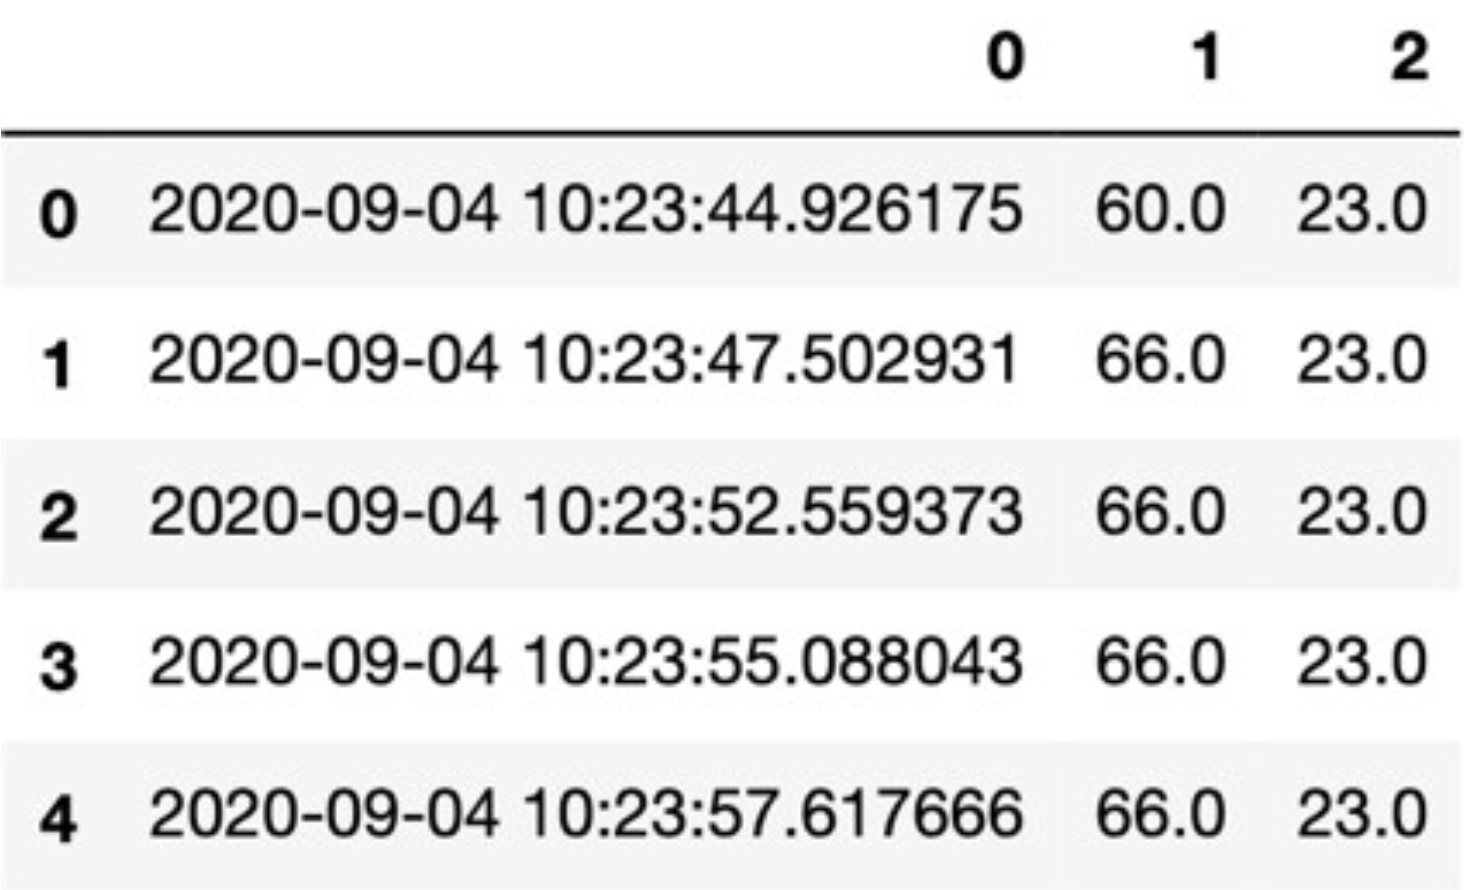
\includegraphics[width=0.5\textwidth]{figures/pandas1.png}\\
    Ovan ser vi att kolumnerna heter 0, 1 och 2, de har alltså bara fått index som namn eftersom det inte fanns några tabellöverskrifter i avsvalningsdatafilen.
    \item Omvandla datum och tid (som är sparat som text) till ett Datetime-objekt så att Python förstår att det är datum och tid. Det gjorde vi i förra labben i kursen med \texttt{pd.to\_datetime()}-funktionen. Nu skall vi utöka vår förmåga att hitta i Pandas-tabeller och använda index för att hitta rätt kolumn. Förutsatt att du har kallat din Pandas dataframe \texttt{cooling} och att \texttt{.head()} ser ut som ovan bör följande uttryck fungera felfritt. 
    (Heter din dataframe något annat, byt bara ut \texttt{cooling} nedan. Vad du kallar din nya kolumn är valfritt, jag använder \texttt{OBJDateTime} för att komma ihåg att det då är Datetime-objekt (alltså riktiga datum och tider och inte text).)    
\begin{lstlisting}[language=Python]
cooling["OBJDateTime"] = pd.to_datetime(cooling.iloc[:,0])\end{lstlisting}
    Här används \texttt{.iloc[]} för att hitta kolumner och rader, där första termen, kolon, inom klamrarna betyder alla rader. Andra termen, 0, betyder första kolumnen (index startar på 0 som vanligt). Till exempel om vi vill ha fjärde raden ges detta av uttrycket: \texttt{cooling.iloc[3,:]}.   Detta behöver ni inte använda, men som förklaring till funktionen \texttt{.iloc[]} passar det som exempel. Testa gärna!
    \item Nu skall du producera två plottar, en för temperatur och en för relativ luftfuktighet. Använd \texttt{.plot()}-funktionen, men måste ges med argument för x och y, annars vet inte Python vad den skall plotta (är blandat text, datum och värden – blir för rörigt och du får felmeddelande). Om du har kallat datumtid-kolumnen från 3 ovan för \texttt{OBJDateTime} bör följande argument ge en plot av luftfuktigheten:
    \begin{lstlisting}[language=Python]
x = "OBJDateTime", y = 1
\end{lstlisting}
    Här är igen inte hela lösningen med, dessa argument skall alltså ges till \texttt{.plot()} på din dataframe. Argumentet för y ges som kolumnindex, för de har inga namn ännu. För att plotta temperaturen byter du bara till \texttt{y = 2}. \hl{\textbf{Dessa två plottar, temperatur mot tid och luftfuktighet mot tid, skall redovisas i din inlämnade PowerPoint så spara dessa separat.}}
    \item I vår modell vill vi bara ha med avsvalningen, men data samlades även innan maxtemperatur har uppnåtts så vi skapar en ny dataframe som börjar då avsvalningen börjar, d.v.s., på sista raden som temperaturen är \SI{60}{\celsius}. Det är lämpligt att spara detta som en egen variabel, som jag nedan kallar \texttt{maxtemp}. Det förutsätts att din dataframe heter \texttt{cooling} och vi använder \texttt{.loc[]} och \texttt{.iloc[]} tillsammans med lite Boolesk logik för att hitta de rader som har temp \qty{60}{\celsius}.
    \begin{lstlisting}[language=Python]
maxtemp = cooling.loc[cooling.iloc[:,2] == 60]
\end{lstlisting}
    Här hittar \texttt{cooling.loc[]} de rader där andra kolumnen (: för alla rader, 2 för kolumn med tempdata) är lika med 60. I min data (den som finns på Blackboard) är detta 15 rader. Om du vill kolla, skriv bara \texttt{maxtemp} i en egen cell och kör den så kommer de raderna upp.
    När vi indexerar i Python kan vi komma åt sista elementet (eller raden, eller kolumnen) genom att använda indexet -1. Alltså om 0 är första indexet och vi inte vet exakt vilket index som är det sista kan vi använda -1. För att hitta sista tillfället då sensorn visar \SI{60}{\celsius} kan vi hitta det med \texttt{.iloc[-1, 3]}, sista raden i fjärde kolumen. Kolumn nummer tre skall vara datetime-objekten om inget har blivit fel. Vi gör en ny dataframe som i exemplet nedan kallas \texttt{cooling\_trunc}, där vi bara har med de tider som är senare och lika med tiden vi hittar med \texttt{.iloc[-1, 3]}:
    \begin{lstlisting}[language=Python]
cooling_trunc = cooling.loc[cooling["OBJDateTime"]
                            >= maxtemp.iloc[-1,3]]
\end{lstlisting}
Här hittar alla rader som är senare (i tid) än sista tiden då sensorn visade 
\qty{60}{\degreeCelsius}. 
\texttt{cooling\_trunc} är en ny dataframe som innehåller 
samma kolumner som \texttt{cooling} men saknar de rader innan sista gången sensorn 
mätte \qty{60}{\celsius}. För att kolla att allt är OK kan vi använda 
\texttt{.head()}, alltså bör \texttt{cooling\_trunc.head()} ge:\\
    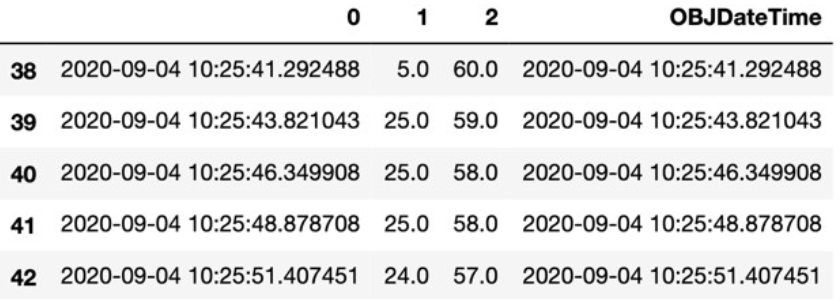
\includegraphics[width=0.75\textwidth]{figures/pandas2.png}\\
    Där vi ser att första raden har temp \SI{60}{\celsius} men sen sjunker temperaturen på nästa mätning. Indexkolumnen börjar på 38 i bilden ovan vilket betyder att vi har klippt bort 38 rader från orginaldatan (första raden är rad 0!). Går att indexera om så den börjar på 0 men det är inte nödvändigt för att fortsätta så vi kan lämna det som det är.
    \item I en modell för avsvalningen vill vi inte ha datum och tid på den horisontella axeln utan vi vill ha antal sekunder startandes på noll och fortsätter räkna i bara sekunder och inte gå över till minuter efter 60 sekunder. För att göra detta subtraherar vi tiden som vår nya dataframe börjar på från alla tidsangivelser i hela kolumnen. Eftersom vi har våra tider som datetime-objekt är detta lätt, bara att använda minus för subtraktion! På denna använder vi metoden \texttt{.dt.total\_seconds()} så får vi det i sekunder endast (inga minuter). Kommandot nedan ger en en-kolumns dataframe med bara sekunder:
    \begin{lstlisting}[language=Python]
timecopy = (cooling_trunc["OBJDateTime"]
            - maxtemp.iloc[-1,3]).dt.total_seconds()
\end{lstlisting}
    Nu är vi nästan på mållinjen för vårt dataset med avsvalningsdata, för att undvika \texttt{SettingWithCopyWarning} (den rosa som förvirrar oss i onödan) gör vi nu en ny dataframe med snygga kolumnnamn där bara förlupen tid i sekunder är med. För att skapa en ny, tom dataframe (som här kallas \texttt{cooling\_small}):
    \begin{lstlisting}[language=Python]
cooling_small = pd.DataFrame()
\end{lstlisting}
    Sedan fyller vi på denna med de kolumner vi behöver (bara förlupen tid i sekunder, \texttt{timecopy} ovan, och temperaturen i kolumn med index 2 från \texttt{cooling\_trunc}):
    \begin{lstlisting}[language=Python]
cooling_small["Time"] = timecopy
cooling_small["Temp"] = cooling_trunc.iloc[:,2]
\end{lstlisting}
    \item \hl{Plotta avsvalningskurvan med tid i sekunder (utan minuter) på x-axeln och temperaturen på y-axeln. \textbf{Denna plot skall redovisas på din PowerPoint-inlämning.}}
\end{enumerate}

\subsection{Lineär regression -- rät linje}
Denna övning bör göras i samma Jupyter-notebook som datainläsningen och -polerandet i övningen ovan. Tänk på att om du stänger av Jupyter-systemet så måste du köra samtliga celler i notebooken när du startar igen så att all data och det du har gjort med den är inläst i datorn så du kan använda det i övningen nedan.

Enklare trender modelleras med en lineär funktion, alltså ett rakt streck. Vårt första försök att skapa en modell och träna på vår avsvalningsdata blir en lineär modell – lineär regression som det heter på statistik- eller för den delen maskininlärningsspråk. Kom ihåg att en lineär funktion ser ut så här:
\[y = k \cdot x + m\]
där $y$  är vårt sökta resultat, i vårt fall ovan är det temperaturen. $x$ är vår oberoende variabel vilket i vårt avsvalningsexperiment motsvarar tiden. Att $x$ är vår oberoende variabel kan vara lite svårt att ta till sig, men det betyder att det är den som \emph{styr}. Det som ändras är tiden (försök stoppa den om du vågar!) och när tiden går sjunker temperaturen. De parametrar som vi har i vår modell är $k$, lutningen på linjen, och $m$, var den skär den vertikala axeln. Dessa två parametrar skall maskininlärningsalgoritmerna ändra på så att linjen passar vår data så bra som möjligt.
\begin{enumerate}
    \item För att göra detta behöver vi lite fler verktyg i vår verktygslåda, för att göra den lineära modellen använder vi modulen LinearRegression från Scikit Learn. Importera denna till din Jupyter notebook på liknande sätt som tidigare. I samma cell kan du importera modulen numpy så vi har tillgång till dess funktionalitet:
    \begin{lstlisting}[language=Python]
from sklearn.linear_model import LinearRegression
import numpy as np
\end{lstlisting}
    \item Vi hämtar ut vår oberoende variabel $X$ (tiden) och vårt resultat $y$ (temperaturen) från vår dataframe som skapades i övningen ovan med kommandona nedan. \texttt{np.vstack()} används för att göra rena kolumner, Scikit-learn vill inte ha Pandas-kolumner.
    \begin{lstlisting}[language=Python]
X = np.vstack(cooling_small["Time"])
y = np.vstack(cooling_small["Temp"])
\end{lstlisting}
    \item Nu är nästa steg att göra själva maskininlärandet (vifta med trollstaven), alltså skapa en modell och skapa prediktioner om temperaturen baserat på vår skapade modell. Vi skapar modellen med minsta kvadratmetoden (som vi nu nästan kan):
    \begin{lstlisting}[language=Python]
model1 = LinearRegression().fit(X, y)
\end{lstlisting}
    Nu har vi skapat vår modell och behöver göra prediktioner med denna av temperaturen:
    \begin{lstlisting}[language=Python]
y_predict1 = model1.predict(X)
\end{lstlisting}
    Här har vi alltså sparat den tränade modellen i kolumnen vi kallar \texttt{y\_predict1}, $y$ för att det är $y$-värden (output), predict för att det är prediktioner och 1 (etta) efteråt för att det är en lineär modell (ett rakt streck). Färdigtrollat! Applåder!
    \item Nästa steg är att kontrollera hur bra modellen blev, det finns flera bra mått på hur bra en modell är, vi kommer här använda oss av absoluta medelfelet, \emph{mean absolute error} (MAE). Dessutom kommer vi plotta data och modell jämte varandra för att få en visuell jämförelse av vad vårt MAE-värde betyder. Funktionen MAE behvöver vi importera från Scikit Learn:
    \begin{lstlisting}[language=Python]
from sklearn.metrics import mean_absolute_error
\end{lstlisting}
    För att beräkna, ger vi funktionen våra riktiga $y$-värden och våra predikterade $y$-värden, \texttt{print()}-kommandot gör så att MAE för vår modell skrivs ut:
    \begin{lstlisting}[language=Python]
mae_linear = mean_absolute_error(y, y_predict1)
print(mae_linear)
\end{lstlisting}
    Bör bli strax under 4.
    \item Sista steget är att plotta data och modell i en liten figur. Nu har vi modellen och vår data i olika tabeller så för detta är det lättast att använda modulen Matplotlib, importera denna så här till din Jupyter notebook:
    \begin{lstlisting}[language=Python]
import matplotlib.pyplot as plt        '
\end{lstlisting}
    Att göra en plot med Matplotlib är ganska lätt, vi använder funktionen \texttt{plt.plot()} eller \texttt{plt.scatter()} med lämpliga argument. Nedan är den första raden vår data från och andra raden plottar modellen som ett streck. Tredje till femte raden lägger till text så att det ser snyggt ut och så att all information finns i figuren. Kommandot \texttt{plt.show()} visar plotten i en figur.
    \begin{lstlisting}[language=Python]
plt.scatter(X, y)
plt.plot(X, y_predict1, 'r')
plt.xlabel("Tid (s)")
plt.ylabel("Temperatur ($^\circ$C)")
plt.legend(["Model","Data" ])
plt.show()
\end{lstlisting}
    \item \hl{\textbf{Redovisa ditt MAE-värde och din figur som visar data och lineär modell i din PowerPoint-inlämning.}}
\end{enumerate}
\subsection{Lineär regression -- kvadratisk modell}
En kvadratisk modell innebär en böjd kurva och eftersom avsvalningen är typiskt böjd bör denna passa något bättre än ett rakt streck. Kvadratisk innebär att det är någonting upphöjt till två, t.ex.
\[ y = \alpha \cdot x^2 + k \cdot x + m \]
Vi skall igen använda Scikit Learn och \texttt{LinearRegression} för att göra regressionen men vi behöver lite andra verktyg för att komma ända dit. Den största skillnaden är att vi behöver göra om våra $X$-värden från ovan med hjälp av en annan modul från Scikit learn, som heter \texttt{PolynomialFeatures}, för att få till en kvadratisk modell.
Du kan fortsätta denna övning i samma Jupyter notebook som övningen ovan, vi kommer använda samma data för denna modell.
\begin{enumerate}
    \item Först importerar vi modulen PolynomialFeatures från Scikit learn:
    \begin{lstlisting}[language=Python]
from sklearn.preprocessing import PolynomialFeatures
\end{lstlisting}
    Sedan bestämmer vi kvadratisk genom göra en modell där vi sätter \texttt{degree = 2} (rad ett nedan), därefter gör vi om våra $X$-värden så de passar i en polynom-modell (rad två nedan):
    \begin{lstlisting}[language=Python]
poly2 = PolynomialFeatures(degree=2)
x_poly2 = poly2.fit_transform(X)
\end{lstlisting}
    \item Efter denna omvandling kör vi på med \texttt{LinearRegresssion} på samma sätt som i övningen ovan, andra raden tränar vår kvadratiska modell.
    \begin{lstlisting}[language=Python]
model2 = LinearRegression().fit(x_poly2, y)
y_predict2 = model2.predict(x_poly2)
\end{lstlisting}
    Där \texttt{model2} blir den kvadratiska modellen (något upphöjt till två), vi har samma $y$-värden (temperaturen är samma) men vi har ändrat $X$-värdena något för att passa en kvadratisk modell.
    \item \hl{Plotta data och prediktioner på samma sätt som i övningen ovan, ta fram MAE med \texttt{mean\_absolute\_error()}. Behöver då givetvis vara med argumentet \texttt{y\_predict2}. \textbf{Redovisa MAE och din figur med data och kvadratisk modell på din PowerPoint- inlämning.}}
\end{enumerate}
\subsection{Modeller av högre ordning ($x^3$ och $x^4$)}
Efter att vi har testat lineär och kvadratisk modell (upphöjt till två) skall vi nu testa modeller av högre ordning. Högre ordning betyder att det är upphöjt till ett större tal än två, vi nöjer oss med att testa tre och fyra.

Jämfört med övning övningarna ovan är det inte speciellt mycket nytt som behöver skrivas, behåll i samma Jupyter notebook och gör en ny cell för $x^3$- och en för $x^4$-modellen. Nedan följer en generell beskrivning som passar bägge dessa, det enda som behöver bytas ut är en trea mot en fyra. Det vi behöver ändra är:
\begin{lstlisting}[language=Python]
poly3 = PolynomialFeatures(degree=3)
\end{lstlisting}
Denna ger oss modell med upphöjt till tre (eller fyra om trean byts ut).
\begin{lstlisting}[language=Python]
x_poly3 = poly3.fit_transform(X)
model3 = LinearRegression().fit(x_poly3, y)
y_predict3 = model3.predict(x_poly3)
\end{lstlisting}
\hl{Plotta data och prediktioner på samma sätt, och ta fram MAE.
För bägge dessa modeller ($x^3$ och $x^4$):
\textbf{Redovisa MAE och din figur med data och modeller på din PowerPoint-inlämning.}}
\subsection{Modelltestning utanför dataområdet}
Sista modellen vi provade, $x^4$, hade när jag gjorde den lågt MAE och följde exempeldatan väldigt väl. Nu skall vi utforska den modellen om vi tänker att tiden tickar på. Vad vi förväntar oss är att modellen förutspår att det kommer fortsätta vara rumstemperatur efter några timmar. Hittills har vi bara gjort prediktioner baserat på våra faktiska, uppmätta $X$-värden 
(ursprungligen från \verb|cooling_small["Time"]|). 
Men dessa sträcker sig bara exakt lika långt som våra mätningar (eftersom varje tid är från en mätning). Vi måste alltså nu skapa en egen kolumn med tider som sträcker sig några timmar, stoppa in i vår modell med lägst MAE och kolla temperaturen efter några timmar baserat på vår modell. Fortsätt i samma Jupyter notebook.
\begin{enumerate}
    \item Det som är nytt i denna övning är att vi skall generera en Numpy-array som startar på \qty{0}{\s} och slutar efter kanske två timmar. Resten är i stort sett samma som delarna ovan. En timme innehåller \qty{3600}{\s}, så om vi kör på till \qty{5000}{\s} eller \qty{7000}{\s} borde vi få se om modellen visar några andra trender än att behålla rumstemperatur. Vi skall använda Numpy-funktionen \texttt{np.linspace()} för att generara ett jämnt intervall av värden och \texttt{np.vstack()} för att de skall stå på rätt håll, parametrar till dessa enligt nedan. Här gör vi direkt våra $X$-värden som krävs för våren modell med av fjärde ordningen och sedan gör vi vår prediktion:
    \begin{lstlisting}[language=Python]
xtest = poly4.fit_transform(np.vstack(
                            np.linspace(0, 5000, 100)))
predictiontest = model4.predict(xtest)
\end{lstlisting}
    \item Plotta datan gör vi som ovan, men plotta vår prediktion blir lite annorlunda eftersom vi måste ange vår \texttt{xtest} som $X$-värden:
    \begin{lstlisting}[language=Python]
plt.scatter(X, y)
plt.plot(xtest[:,1], predictiontest, 'r')
\end{lstlisting}
    \texttt{xtest[:,1]} behövs för våra $X$-värden har fått lite fler kolumner när vi transformerar om dem med \texttt{PolynomialFeatures}.
    \item \hl{\textbf{Klistra in den figuren i din Powerpoint tillsammans med sluttemperaturen.}} Sluttemperaturen kan fås direkt som sista värdet i \texttt{predictiontest}, alltså då tiden har nått \qty{5000}{\s} (eller vilken tid du nu valde) via: 
    \begin{lstlisting}[language=Python]
predictiontest[-1]
\end{lstlisting}
    Sista värdet som index i Python är alltid -1. (Näst sista -2 etc.)
\end{enumerate}
\subsection{Regressionsträd för stabilare modell}
Beroende på vilken data du använde övningarna ovan gav vissa av de olika modellerna ganska dåliga resultat. I den här övningen skall du testa att göra en modell baserat på regressionsträd, alltså en variant av beslutsträd (decision trees) som används för att göra en modell av en kurva. Använd i den här delen det något större datasettet \texttt{cooling\_data\_BPA.txt} som finns på Blackboard.
\begin{enumerate}
    \item Dela tränings- och testdata. Här behövs tre moduler från Scikit learn: \texttt{train\_test\_split} för att dela upp datan i tränings- och testdata,\\ \texttt{DecisionTreeRegression} för att göra själva modellen och igen\\ \texttt{mean\_absolute\_error} för att testa om modellen är bra. Vi behöver även Numpy för att konvertera datan från dataframe. Importera de nya på följande sätt:
    \begin{lstlisting}[language=Python]
from sklearn.tree import DecisionTreeRegressor
from sklearn.model_selection import train_test_split
\end{lstlisting}
    För att dela upp datan i tränings- och testdata använder vi följande kommando:
    \begin{lstlisting}[language=Python]
X_train, X_test, y_train, y_test = train_test_split(
                                np.vstack(multidata["Time"]), 
                                np.vstack(multidata["Temp"]), 
                                test_size = 0.3, 
                                shuffle = True)    
\end{lstlisting}
    Till vänster om likhetstecknet ovan skapas variabler som innehåller $X$- och $y$-värden (tid i sekunder och temperatur i \si{\celsius}) fördelat på tränings- och testdata. Till höger om likhetstecknet läses data in, här finns $X$-värdena i kolumnen \texttt{”Time”} i dataframen \texttt{multidata} och $y$-värdena i kolumnen \texttt{”Temp”} i samam dataframe. För att konvertera från dataframes till ren kolumndata används ovan \texttt{np.vstack()}, detta krävs av\\ \texttt{DecisionTreeRegressor}. Heter din dataframe eller kolumnerna något annat behöver dessa ändras. De sista två raderna är mycket viktiga, \texttt{test\_size} bestämmer hur stor del av datan som skall användas för test (30\% i det här fallet) och \texttt{shuffle} väljer slumpmässigt ut de som skall vara test- och träningsdata.
    \emph{Kommandot ovan är bara en rad i Python, jag har lagt in radbryt för att det skall få plats och se lite snyggare ut, men påverkar inte funktionen}.
    \item Träna träd-modellen med \texttt{.fit}:
    \begin{lstlisting}[language=Python]
model_tree = DecisionTreeRegressor(max_depth=5).fit(X_train, y_train)        
\end{lstlisting}
    Här ges den tränade modellen namnet \texttt{model\_tree} till vänster om likhetstecknet. Till höger om likhetstecknet använder vi vår modell, sätter maxantal nivåer i trädet till fem och stoppar in träningsdatan.
    \item Gör prediktion baserat på den tränade modellen och visualisera resultatet.
    \begin{lstlisting}[language=Python]
Xpred = np.vstack(np.linspace(0, 5000, 100))
predictions = model_tree.predict(Xpred)        
\end{lstlisting}
    På första raden ovan skapar vi test-data (\texttt{Xpred}) som innehåller tid från \qty{0}{\s} till \qty{5000}{\s} i 100 steg.
    \item \hl{Visualisera med \texttt{plt.plot} och \texttt{plt.scatter} för modell respektive data. \textbf{Denna plot skall vara med i din PowerPoint-redovisning av datorlaborationerna.}}
    \item Testa hur bra modellen är med hjälp av test-datan. För detta använder vi absoluta medelfelet, det som man får är hur stort felet är i genomsnitt på prediktionen:
    \begin{lstlisting}[language=Python]
mae_train = mean_absolute_error(y_train,
                                model_tree.predict(X_train))
mae_test = mean_absolute_error(y_test,
                               model_tree.predict(X_test))
\end{lstlisting}
    Det är förväntat att felet är ganska lågt på träningsdatan, men kan vara något (eller betydligt) högre på testdatan.
    \hl{\textbf{Redovisa absoluta medelfelet för både tränings och testdata på din PowerPoint.}}
\end{enumerate}

%\section{Klassificering och beslutsträd från grunden}
%I den här labben kommer vi ge er en grundläggande förståelse för ett av de vanligare verktygen när det kommer till klassificering inom Machine Learning, nämligen Decision Trees. Men innan vi går in mer på Decision Trees så kommer en kort genomgång av vad klassificering innebär. 
%Inom Machine Learning så är de vanligaste typernena antingen Regression eller Klassificering. Enkelt sätt så kan man säga att Regression handlar om kontinuerliga värden, medan Klassificering handlar om att bestämma något som en förbestämd klass. Ett exempel till Regression skulle kunna vara att förutspå huspriser baserat på storlek, medans ett exempel på klassificering skulle vara att säga om ett djur på en bild är antingen en hund eller katt.
%Det finns flera olika algorithmer att använda inom Klassificering, i denna labben kommer vi att använda något som kallas Decision Tree. Ett Decision tree kan enkelt beskrivas som en sekvens av Ja eller Nej frågor för att leda fram till en slutsats.
%
%\begin{figure}[h]
%    \centering
%    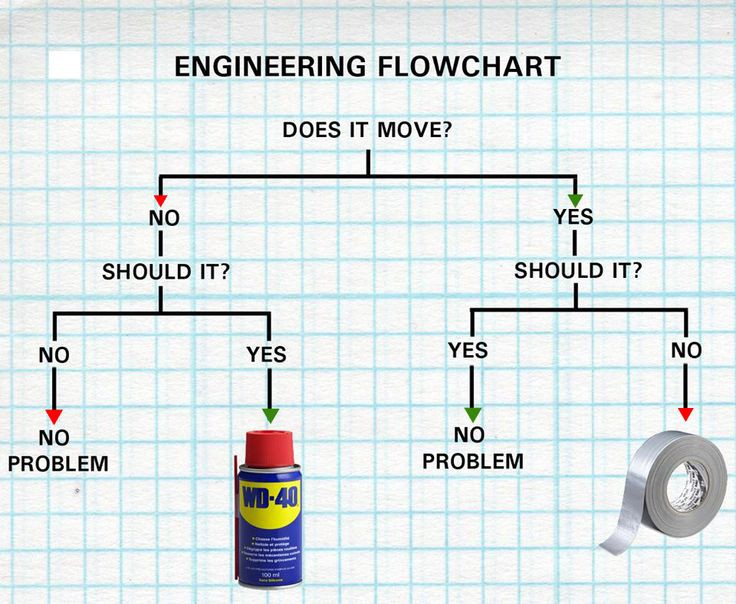
\includegraphics[scale = 0.3]{dtex.jpeg}
%    \caption*{Ett exempel på ett decision tree}
%    \label{fig:dtex}
%\end{figure}
%
%\subsection{Regressionsträdsprogrammering}
%I denna labben skall ni bygga ert eget träd från grunden, istället för att använda färdiga moduler eller bibliotek. Detta görs enklast med en sekvens utav $if-satser$. Ni skall ta data från en utav SMHIs väderstationer och sedan använda SMHIs definitioner för när en årstid börjar för att kunna kategorisera ett datum som antingen Vår, Sommar, Vinter eller Höst. Eftersom SMHIs definitioner pekar på när en viss årstid börjar så kan det bli lite roliga resultat! 
%
%SMHIs definitioner lyder som följande.
%
%\begin{itemize}
%    \item Vinter: 5 dygn i följd med temperatur under 0 grader.
%    \item Vår: 7 dagar i följd med temperatur över 0 grader, men inte senare än 31 Juli
%    \item Sommar: 5 dagar i följd med temperatur över 10 grader.
%    \item Höst: 5 dagar i följd med temperatur under 10 grader, men inte innan 1 Augusti.
%    
%\end{itemize}
%
%Det ert program skall göra är att det ska ta ett datum som en input, kolla sedan på $x$ (5 eller 7) antal dagar innan detta datumet för att bedömma vilken meteorologisk årstid som passar bäst in på ditt datum!
%Den enda datan ni behöver från SMHI är medeltemperatur för dagen samt datum!

\section{Klimatförändringar -- återbesök av SMHI-data}
I den här övningen skall du använda de SMHI-data som du hämtade och gjorde lite statistisk analys på i förra labben. Du skall i denna övning använda din historiska data över medeltemperaturen i juli för att prediktera medeltemperaturen i juli 2030 baserat på en lineär regressionsmodell. Rekommenderat är att du skapar en ny Jupyter notebook och kopierar över inläsningen av SMHI-datan från din notebook i förra delen av kursen till den nya. Kom ihåg att notebooken och datan behöver ligga i samma katalog på datorn för att det skall fungera.
\begin{enumerate}
    \item Skapa en ny dataframe som innehåller bara juli-data. Beroende på vad du döper dina dataframes till kan raden nedan användas för att skapa denna dataframe. Kom ihåg att du behöver ha gjort om datum i textformat till datum i DateTime-objekt-format för att det skall fungera (görs med \texttt{pd.to\_datetime()}-funktionen)
    \begin{lstlisting}[language=Python]
juliT = smhidata_datum.loc[pd.DatetimeIndex(
                        smhidata_datum["OBJDatum"]).month==7]        
\end{lstlisting}
    Här är \texttt{juliT} min dataframe med bara julidata och \texttt{smhidata\_datum} är min dataframe med temperaturdata från samtliga år som fanns med. Efter denna behandling bör din dataframe med bara juli-data se ut något i stil med:\\
    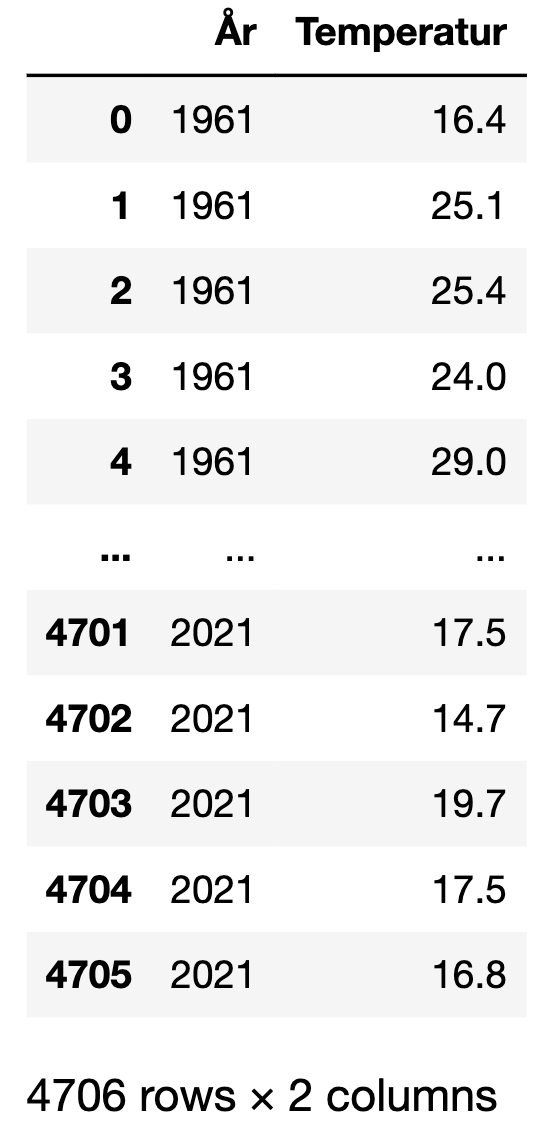
\includegraphics[width=0.3\textwidth]{figures/julitemp.png}
    \item Nu behöver du bara sortera på år och ta medelvärdet sen är du redo att förutspå klimatförändringar. Pandas har en smart funktion som heter \texttt{.groupby()} som är högst användbar här. Går givetvis att lösa med en loop eftersom det inte är så många datapunkter det handlar om. För att skapa en mindre, grupperad dataframe med medeltemperaturen i juli varje år bör följande fungera (beroende på vad dina dataframes och kolumner heter):
    \begin{lstlisting}[language=Python]
datat = julitemp.groupby("Year").mean()
\end{lstlisting}
    Här grupperar Pandas på årtal och tar medelvärdet av varje år. Följande rader visar de fem första raderna, de fem sista raderna och en plot på årtal.  
    \begin{lstlisting}[language=Python]
display(datat.head(), datat.tail())
datat.plot()
plt.show()
\end{lstlisting}
    Inklippt blir det så här:\\
    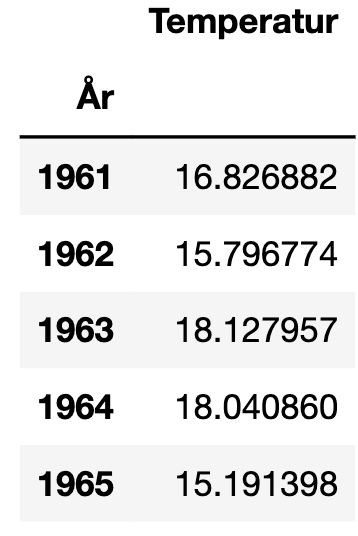
\includegraphics[width=0.25\textwidth]{figures/Screenshot 2022-11-18 at 10.47.20.png}
    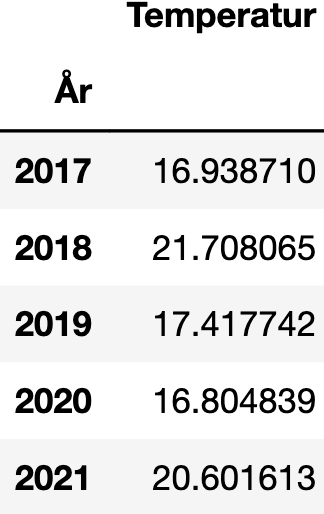
\includegraphics[width=0.235\textwidth]{figures/Screenshot 2022-11-18 at 10.47.29.png}
    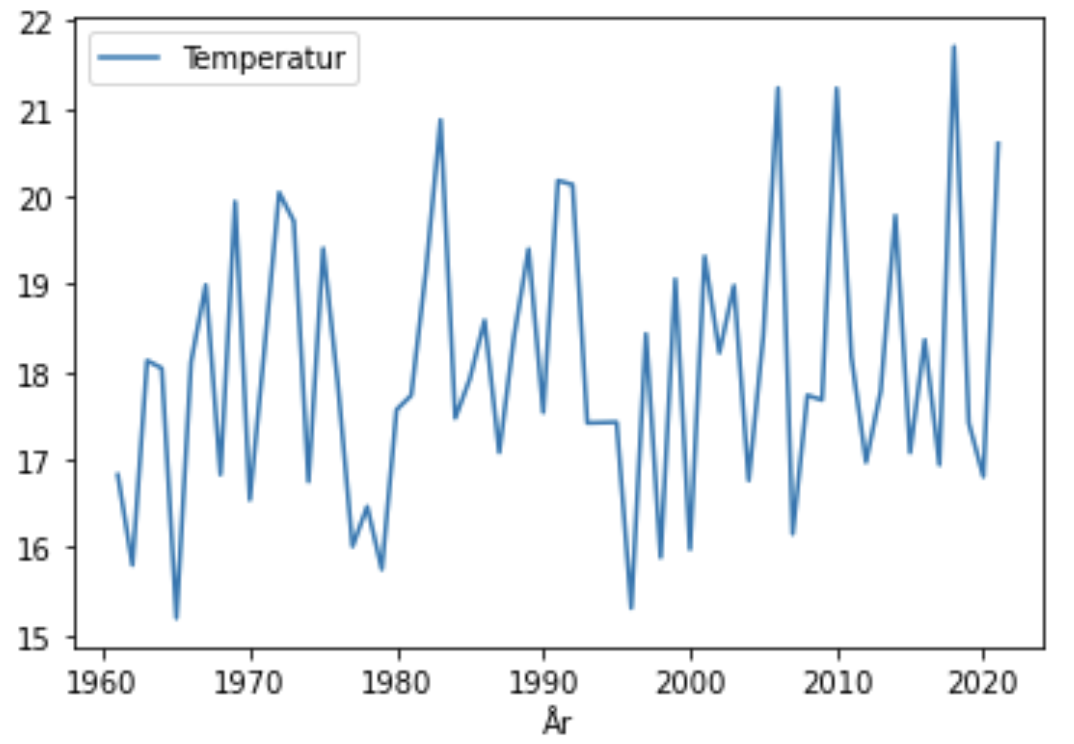
\includegraphics[width=0.45\textwidth]{figures/Screenshot 2022-11-18 at 10.47.37.png}   \\
    Givetvis beroende på vilken väderstation du har valt, detta är för Oskars\-hamn.
    \item Gör en lineär regressionsmodell för temperaturen över de år som finns i din SMHI- data. Det gör du på liknande sätt som i övningen med lineär regression ovan.

    \hl{\textbf{I din PowerPoint-inlämning för denna övning skall data- och regressionsplot, predikterad temperatur år 2030 och MAE för din modell vara med.}} \\
    För att prediktera temperaturen år 2030 behöver vi kalla:
    \begin{lstlisting}[language=Python]
model1.predict(np.vstack([2030]))
\end{lstlisting}
    Förutsatt att din modell av medeltemperaturen i juli heter \texttt{model1}.
\end{enumerate}
\pagebreak
\section{Grand finale}\label{grandfinale}
Kronan på verket i den här kursen är att du skall som Data Scientist kontrollera isolationen i din bostad (i alla fall på ett ungefär). Nu skall du samla in temperaturdata inomhus och göra en jämförelse med SMHIs utomhusdata för samma tidsperiod för att avgöra om isoleringen är bra eller dålig. I princip består denna uppgift av tre uppgifter, datainsamling, datarensande och datapresentation.
\begin{enumerate}
    \item Samla in temperaturdata inomhus med din Raspberry över \textbf{lite längre tidsperiod}, typiskt en eller två veckor men \textbf{minimum två dygn}. Ladda ner datan från Thingspeak. 
    \item Ladda ner SMHI-data för samma tidsperiod som i punkten ovan, observera att SMHI har senaste tre månaderna och historiska data (äldre än tre månader) i olika filer eftersom SMHI kvalitetskontrollerar innan de lägger till i den historiska datan. 
    \item Nu bör du besitta tillräckliga kunskaper för att göra snygga dataset med datum, tid, inomhus- och utomhustemperatur. Bestäm själv hur ofta du vill mäta, men det kommer vara SMHI som sätter gränsen där eftersom stationerna inte mäter (eller i alla fall inte sparar) datan jätteofta. Medelvärdet på temperaturen per timme bör räcka. \hl{\textbf{I din PowerPoint-inlämning bör \texttt{.head()} på din slutliga dataframe vara med.}}
    \item \hl{Briljera med dina Data Science-kunskaper och \textbf{ha med den snyggaste visualiseringen du kan uppbåda på din ute- och inomhustemperatur} samt korrelationen mellan dessa. Visualiseringen \textbf{skall} vara både temperaturer mot datum OCH inomhustemp mot utomhustemp. }
\end{enumerate}
\end{document}
